% Created 2020-09-18 fr 10:13
% Intended LaTeX compiler: pdflatex
\documentclass[12pt]{article}

%%%% settings when exporting code %%%% 

\usepackage{listings}
\lstset{
backgroundcolor=\color{white},
basewidth={0.5em,0.4em},
basicstyle=\ttfamily\small,
breakatwhitespace=false,
breaklines=true,
columns=fullflexible,
commentstyle=\color[rgb]{0.5,0,0.5},
frame=single,
keepspaces=true,
keywordstyle=\color{black},
literate={~}{$\sim$}{1},
numbers=left,
numbersep=10pt,
numberstyle=\ttfamily\tiny\color{gray},
showspaces=false,
showstringspaces=false,
stepnumber=1,
stringstyle=\color[rgb]{0,.5,0},
tabsize=4,
xleftmargin=.23in,
emph={anova,apply,class,coef,colnames,colNames,colSums,dim,dcast,for,ggplot,head,if,ifelse,is.na,lapply,list.files,library,logLik,melt,plot,require,rowSums,sapply,setcolorder,setkey,str,summary,tapply},
emphstyle=\color{blue}
}

%%%% packages %%%%%

\usepackage[utf8]{inputenc}
\usepackage[T1]{fontenc}
\usepackage{lmodern}
\usepackage{textcomp}
\usepackage{color}
\usepackage{enumerate}
\usepackage{graphicx}
\usepackage{grffile}
\usepackage{wrapfig}
\usepackage{rotating}
\usepackage{longtable}
\usepackage{multirow}
\usepackage{multicol}
\usepackage{changes}
\usepackage{pdflscape}
\usepackage{geometry}
\usepackage[normalem]{ulem}
\usepackage{amssymb}
\usepackage{amsmath}
\usepackage{amsfonts}
\usepackage{dsfont}
\usepackage{array}
\usepackage{ifthen}
\usepackage{hyperref}
\usepackage{natbib}
%
%%%% specifications %%%%
%
\usepackage{ifthen}
\usepackage{xifthen}
\usepackage{xargs}
\usepackage{xspace}
\newcommand\Rlogo{\textbf{\textsf{R}}\xspace} %
\RequirePackage{fancyvrb}
\DefineVerbatimEnvironment{verbatim}{Verbatim}{fontsize=\small,formatcom = {\color[rgb]{0.5,0,0}}}
\RequirePackage{colortbl} % arrayrulecolor to mix colors
\RequirePackage{setspace} % to modify the space between lines - incompatible with footnote in beamer
\renewcommand{\baselinestretch}{1.1}
\geometry{top=1cm}
\RequirePackage{epstopdf} % to be able to convert .eps to .pdf image files
\RequirePackage{capt-of} %
\RequirePackage{caption} % newlines in graphics
\RequirePackage{amsmath}
\RequirePackage{algorithm}
\RequirePackage[noend]{algpseudocode}
\RequirePackage{dsfont}
\RequirePackage{amsmath,stmaryrd,graphicx}
\RequirePackage{prodint} % product integral symbol (\PRODI)
\newcommand\defOperator[7]{%
\ifthenelse{\isempty{#2}}{
\ifthenelse{\isempty{#1}}{#7{#3}#4}{#7{#3}#4 \left#5 #1 \right#6}
}{
\ifthenelse{\isempty{#1}}{#7{#3}#4_{#2}}{#7{#3}#4_{#1}\left#5 #2 \right#6}
}
}
\newcommand\defUOperator[5]{%
\ifthenelse{\isempty{#1}}{
#5\left#3 #2 \right#4
}{
\ifthenelse{\isempty{#2}}{\underset{#1}{\operatornamewithlimits{#5}}}{
\underset{#1}{\operatornamewithlimits{#5}}\left#3 #2 \right#4}
}
}
\newcommand{\defBoldVar}[2]{
\ifthenelse{\equal{#2}{T}}{\boldsymbol{#1}}{\mathbf{#1}}
}
\newcommandx\Cov[2][1=,2=]{\defOperator{#1}{#2}{C}{ov}{\lbrack}{\rbrack}{\mathbb}}
\newcommandx\Esp[2][1=,2=]{\defOperator{#1}{#2}{E}{}{\lbrack}{\rbrack}{\mathbb}}
\newcommandx\Prob[2][1=,2=]{\defOperator{#1}{#2}{P}{}{\lbrack}{\rbrack}{\mathbb}}
\newcommandx\Qrob[2][1=,2=]{\defOperator{#1}{#2}{Q}{}{\lbrack}{\rbrack}{\mathbb}}
\newcommandx\Var[2][1=,2=]{\defOperator{#1}{#2}{V}{ar}{\lbrack}{\rbrack}{\mathbb}}
\newcommandx\Binom[2][1=,2=]{\defOperator{#1}{#2}{B}{}{(}{)}{\mathcal}}
\newcommandx\Gaus[2][1=,2=]{\defOperator{#1}{#2}{N}{}{(}{)}{\mathcal}}
\newcommandx\Wishart[2][1=,2=]{\defOperator{#1}{#2}{W}{ishart}{(}{)}{\mathcal}}
\newcommandx\Likelihood[2][1=,2=]{\defOperator{#1}{#2}{L}{}{(}{)}{\mathcal}}
\newcommandx\Information[2][1=,2=]{\defOperator{#1}{#2}{I}{}{(}{)}{\mathcal}}
\newcommandx\Score[2][1=,2=]{\defOperator{#1}{#2}{S}{}{(}{)}{\mathcal}}
\newcommandx\Vois[2][1=,2=]{\defOperator{#1}{#2}{V}{}{(}{)}{\mathcal}}
\newcommandx\IF[2][1=,2=]{\defOperator{#1}{#2}{IF}{}{(}{)}{\mathcal}}
\newcommandx\Ind[1][1=]{\defOperator{}{#1}{1}{}{(}{)}{\mathds}}
\newcommandx\Max[2][1=,2=]{\defUOperator{#1}{#2}{(}{)}{min}}
\newcommandx\Min[2][1=,2=]{\defUOperator{#1}{#2}{(}{)}{max}}
\newcommandx\argMax[2][1=,2=]{\defUOperator{#1}{#2}{(}{)}{argmax}}
\newcommandx\argMin[2][1=,2=]{\defUOperator{#1}{#2}{(}{)}{argmin}}
\newcommandx\cvD[2][1=D,2=n \rightarrow \infty]{\xrightarrow[#2]{#1}}
\newcommandx\Hypothesis[2][1=,2=]{
\ifthenelse{\isempty{#1}}{
\mathcal{H}
}{
\ifthenelse{\isempty{#2}}{
\mathcal{H}_{#1}
}{
\mathcal{H}^{(#2)}_{#1}
}
}
}
\newcommandx\dpartial[4][1=,2=,3=,4=\partial]{
\ifthenelse{\isempty{#3}}{
\frac{#4 #1}{#4 #2}
}{
\left.\frac{#4 #1}{#4 #2}\right\rvert_{#3}
}
}
\newcommandx\dTpartial[3][1=,2=,3=]{\dpartial[#1][#2][#3][d]}
\newcommandx\ddpartial[3][1=,2=,3=]{
\ifthenelse{\isempty{#3}}{
\frac{\partial^{2} #1}{\partial #2^2}
}{
\frac{\partial^2 #1}{\partial #2\partial #3}
}
}
\newcommand\Real{\mathbb{R}}
\newcommand\Rational{\mathbb{Q}}
\newcommand\Natural{\mathbb{N}}
\newcommand\trans[1]{{#1}^\intercal}%\newcommand\trans[1]{{\vphantom{#1}}^\top{#1}}
\newcommand{\independent}{\mathrel{\text{\scalebox{1.5}{$\perp\mkern-10mu\perp$}}}}
\newcommand\half{\frac{1}{2}}
\newcommand\normMax[1]{\left|\left|#1\right|\right|_{max}}
\newcommand\normTwo[1]{\left|\left|#1\right|\right|_{2}}
\author{Brice Ozenne}
\date{\today}
\title{Diagnostics and partial residuals in a linear model}
\hypersetup{
 colorlinks=true,
 citecolor=[rgb]{0,0.5,0},
 urlcolor=[rgb]{0,0,0.5},
 linkcolor=[rgb]{0,0,0.5},
 pdfauthor={Brice Ozenne},
 pdftitle={Diagnostics and partial residuals in a linear model},
 pdfkeywords={},
 pdfsubject={},
 pdfcreator={Emacs 25.2.1 (Org mode 9.0.4)},
 pdflang={English}
 }
\begin{document}

\maketitle

\section*{Summary}
\label{sec:orgfc8d9ca}
In the document we provide a brief introduction to the linear model
and its underlying assumptions. We then show how some of these
hypotheses can be checked and what to do when there is evidence that
one or several assumptions are not met. Finally we introduce the
notion of partial residuals and explain how to compute and display
them.

\bigskip

To be able to run the R code you will need to load the following
packages:
\lstset{language=r,label= ,caption= ,captionpos=b,numbers=none}
\begin{lstlisting}
library(lava) ## install.packages("lava")
library(car) ## install.packages("car")
library(nlme) ## install.packages("nlme")
library(butils) ## devtools::install_github("bozenne/butils")
library(gof) ## devtools::install_github("kkholst/gof")
library(ggfortify) ## install.packages("ggfortify")
\end{lstlisting}

The first is hosted on CRAN and can be install directly. The next two
are hosted on Gihub so you should first install the package devtools
(using \texttt{install.packages}) and then you will be able to install these
packages via the command \texttt{install\_gitub} as shown above (after the
\texttt{\#\#}).

\clearpage

\section{Data}
\label{sec:orge5398e8}

We will use the dataset generated by the following commands:

\lstset{language=r,label= ,caption= ,captionpos=b,numbers=none}
\begin{lstlisting}
set.seed(10)
m.lvm <- lvm(Y[100:sigma2]~beta*AgeC+BMI2+Gene)
categorical(m.lvm, K = 3) <- ~Gene
distribution(m.lvm, ~Age) <- uniform.lvm(20,50)
distribution(m.lvm, ~BMI) <- gaussian.lvm(mean = 24)
transform(m.lvm, AgeC~Age) <- function(x, ...){x-35}
transform(m.lvm, Id~Age) <- function(x, ...){1:NROW(x)}
transform(m.lvm, BMI2~BMI) <- function(x, ...){(x-24) + (x-24)^2}
latent(m.lvm) <- ~AgeC+BMI2
d <- rbind(cbind(lava::sim(n = 1e2, m.lvm, latent=FALSE, p = c(beta = 1, sigma2 = 1)), Gender = "Male"),
		   cbind(lava::sim(n = 1e2, m.lvm, latent=FALSE, p = c(beta = 2, sigma2 = 2)), Gender = "Female")
		   )

d$Gender <- as.factor(d$Gender)
d$Gene <- factor(d$Gene, labels = c("A","B","C"))
d$Y <- round(d$Y,1)
d$Age <- round(d$Age,1)
d$BMI <- round(d$BMI,1)
head(d)
\end{lstlisting}

\begin{verbatim}
      Y Gene  Age  BMI Id Gender
1 115.7    A 48.0 25.2  1   Male
2 108.7    B 42.4 24.3  2   Male
3 108.6    A 41.7 25.4  3   Male
4 104.4    C 36.4 24.9  4   Male
5  93.3    A 27.9 22.9  5   Male
6  97.3    C 29.2 24.5  6   Male
\end{verbatim}

\clearpage

\section{Short introduction to the linear model}
\label{sec:org85783f1}

Imagine we would like to model the age effect on the outcome, but
accounting for a possible gender and gene effect. In \Rlogo{} we would
use the \texttt{lm} function:
\lstset{language=r,label= ,caption= ,captionpos=b,numbers=none}
\begin{lstlisting}
e.lm <- lm(Y~Gender+Age+Gene+BMI, data = d)
e.lm
\end{lstlisting}

\begin{verbatim}

Call:
lm(formula = Y ~ Gender + Age + Gene + BMI, data = d)

Coefficients:
 (Intercept)  GenderFemale           Age         GeneB         GeneC           BMI  
     21.3988        0.9778        1.5326        1.3783        2.6682        1.0351
\end{verbatim}

Denote for the \(i-th\) patient its outcome value by \(Y_i\) (can be
any real number), its gender value by \(Gender_i\) (can be "Male" or
"Female"), its gene value by \(Gene_i\) (can be "A", "B", or
"C"), and its BMI value by \(BMI_i\). Mathematically, this linear model can be written:
\begin{align*}
Y_i =& \alpha + \beta_{Gender} * \Ind[Gender_i="Female"] + \beta_{Age} * Age_i + \beta_{GeneB} *  \Ind[Gene_i="B"] + \beta_{GeneC} * \Ind[Gene_i="C"] \\
& + \beta_{BMI} * BMI_i + \varepsilon_i
\end{align*}
where \(\boldsymbol{\beta} =
(\alpha,\beta_{Gender},\beta_{Age},\beta_{GeneB},\beta_{GeneC},\beta_{BMI})\) is
the vector of model parameters. Their value is shown just above
(e.g. \(\alpha=-21.3988\)). Here \(\Ind[.]\) denotes the indicator
function taking value 1 if "." is true and 0
otherwise. \(\varepsilon_i\) is the residual error, i.e. the
difference between the observed value and the observed value. Consider
for instance the first individual:
\lstset{language=r,label= ,caption= ,captionpos=b,numbers=none}
\begin{lstlisting}
d[1,]
\end{lstlisting}

\begin{verbatim}
      Y Gene Age  BMI Id Gender
1 115.7    A  48 25.2  1   Male
\end{verbatim}
its observed value is 115.7 and we can computed its fitted value as:
\begin{align*}
\hat{Y}_1 &= \alpha + \beta_{Gender} * 0 + \beta_{Age} 48 + \beta_{GeneB} * 0 + \beta_{GeneC} * 0 \\
          &= 21.3988 + 0.9778 * 0 + 1.5326 * 48 + 1.3783 * 0 + 2.6682 * 0 + 1.0351 * 25.2 \\
          & = 121.048
\end{align*}

\clearpage 

This can also be obtained using the \texttt{fitted} method in \Rlogo{} (the
discrepancy comes from rounding the coefficient values at the 4th
digit):
\lstset{language=r,label= ,caption= ,captionpos=b,numbers=none}
\begin{lstlisting}
fitted(e.lm)[1]
\end{lstlisting}

\begin{verbatim}
       1 
121.0474
\end{verbatim}

Often, for conciseness, this linear model can be abbreviated as:
\begin{align*}
Y_i = X_i \boldsymbol{\beta} + \varepsilon_i
\end{align*}
where \(X_i = \left(1, \Ind[Gender_i="Female"], Age_i,
\Ind[Gene_i="B"], \Ind[Gene_i="C"]\right)\) and \(X_i
\boldsymbol{\beta}\) is the matrix product between the row vector
\(X_i\) and the column vector \(\boldsymbol{\beta}\). More generally,
i.e. at the population level instead of the individual level, we also
write \(Y = X \boldsymbol{\beta} + \varepsilon\) to describe the
relationship between the random variables \(Y\), \(X\),
\(\varepsilon\).

\section{Assumptions}
\label{sec:orgd56ea5e}
A linear model \(Y = X \beta + \varepsilon\) is a model studying the
 effects (\(\beta\)) of covariates (\(X\)) on the expected value of
 the outcome \(Y\). Maximum likelihood (ML) estimation leads to
 unbiased estimates of \(\beta\) if the following assumptions are
 satisfied:
\begin{itemize}
\item \textbf{(A0)}: no unobserved confounders.
\item \textbf{(A1)}: \(\Esp[Y_i|X] = X_i \beta\) correct specification of the
functional form of the covariates.
\item \textbf{(A2)}: identically distributed and \textbf{(A3)} independent
residuals. \newline Under the normality assumption, it simplifies to
\textbf{(A2)} homoschedasticity \(\Var[Y_i|X]= \sigma^2\) and \textbf{(A3)}
uncorrelatedness \(\forall i \neq j\), \(\Cov[Y_i,Y_j|X]= 0\).
\end{itemize}
While not needed per se, the assumption of:
\begin{itemize}
\item \textbf{(A4)}: normally distributed residuals is often mentioned since (i)
normality of the estimates holds exactly in finite samples (instead
of asymptotically) i.e. p-values/CIs are reliable even in small
samples, (ii) it ensures that MLE is the best estimation procedure,
(iii) checking \textbf{(A2)} and \textbf{(A3)} is simplified.
\end{itemize}
Additional assumptions are typically necessary to ensure reliable and
interpretable estimates:
\begin{itemize}
\item \textbf{(A4-bis)}: approximately symmetric and unimodal - otherwise modeling the
expected value (aka the mean value) may not be very relevant.
\item \textbf{(A5)}: absence of outliers - otherwise the estimates may be very
sensitive to the value of a few observations which is often
undesirable.
\end{itemize}

\clearpage

\section{Checking assumptions made when fitting a linear model}
\label{sec:orgc5e010e}

\subsection{\textbf{(A0)}: no unobserved confounders}
\label{sec:orge43893f}
\textbf{(A0)} is in general impossible to check.

\subsection{\textbf{(A1)}: correct specification of the functional}
\label{sec:org2dc9d8c}
\textbf{(A1)} can be (artificially) decomposed into two part:
\begin{itemize}
\item in absence of interaction, \textbf{is the effect of the continuous
variables correctly modeled?} Typically it is modeled as a linear
effect and the question is is there a non-linear effect. We can look
at the plot of the covariate vs. the residuals and search for any
trend:
\end{itemize}
\lstset{language=r,label= ,caption= ,captionpos=b,numbers=none}
\begin{lstlisting}
gg <- ggplot(d, aes(x = BMI, y = residuals(e.lm)))
gg <- gg + geom_point() + geom_smooth() + ylab("residuals")
gg
## ggsave(gg + theme(text = element_text(size=25)), filename = "./figures/A1-BMI.pdf")
\end{lstlisting}

\begin{verbatim}
`geom_smooth()` using method = 'loess' and formula 'y ~ x'
\end{verbatim}

\begin{center}
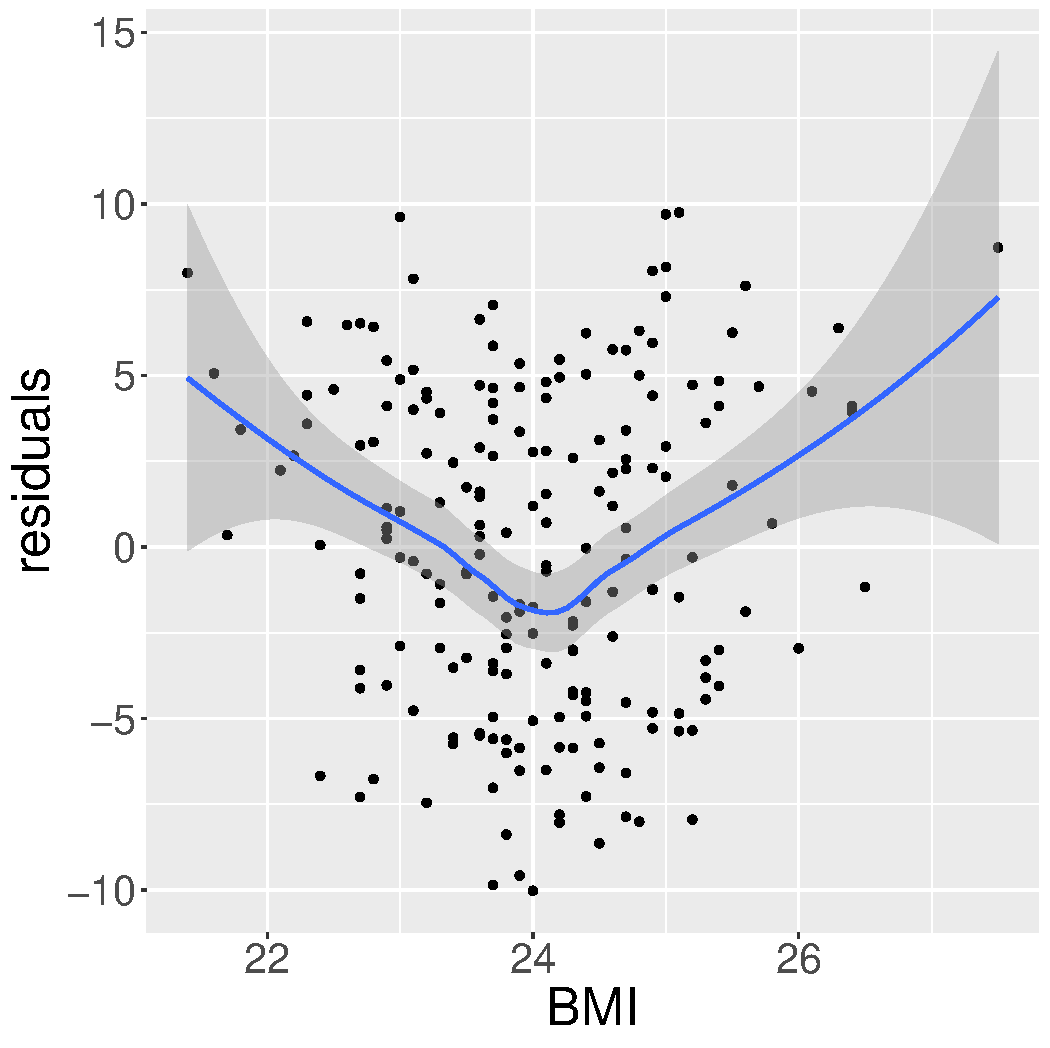
\includegraphics[width=0.7\textwidth]{./figures/A1-BMI.pdf}
\end{center} 

(similar plots can be automatically generated using the \texttt{crPlots} or
\texttt{ceresPlots} function from the car package). A p-value for testing the correct
specification of the functional form for the covariate can be obtained
using the \texttt{cumres} function from the gof package:
\lstset{language=r,label= ,caption= ,captionpos=b,numbers=none}
\begin{lstlisting}
cumres(e.lm, variable = "BMI")
\end{lstlisting}

\begin{verbatim}

Kolmogorov-Smirnov-test: p-value=0.002
Cramer von Mises-test: p-value=0
Based on 1000 realizations. Cumulated residuals ordered by BMI-variable.
---
\end{verbatim}

\emph{Remedies}: if a trend is found, a possible remedy is to use splines to model the
non-linear relationship, e.g. 
\lstset{language=r,label= ,caption= ,captionpos=b,numbers=none}
\begin{lstlisting}
e.gam <- mgcv::gam(Y ~ Gender + Age + Gene + s(BMI), data = d)
\end{lstlisting}
In this simple example, it looks like a quadratic function of BMI
would be enough:
\lstset{language=r,label= ,caption= ,captionpos=b,numbers=none}
\begin{lstlisting}
e.lm.1 <- lm(Y ~ Gender + Age + Gene + BMI + I(BMI^2), data = d)
cumres(e.lm.1, variable = "BMI")
\end{lstlisting}

\begin{verbatim}

Kolmogorov-Smirnov-test: p-value=0.2
Cramer von Mises-test: p-value=0.164
Based on 1000 realizations. Cumulated residuals ordered by BMI-variable.
---
\end{verbatim}
Note that this type of test is not appropriate to detect missing
interaction:
\lstset{language=r,label= ,caption= ,captionpos=b,numbers=none}
\begin{lstlisting}
cumres(e.lm.1, variable = "Age")
\end{lstlisting}

\begin{verbatim}

Kolmogorov-Smirnov-test: p-value=0.274
Cramer von Mises-test: p-value=0.332
Based on 1000 realizations. Cumulated residuals ordered by Age-variable.
---
\end{verbatim}
while the display of the residuals can be informative
\lstset{language=r,label= ,caption= ,captionpos=b,numbers=none}
\begin{lstlisting}
gg <- ggplot(d, aes(x = Age, y = residuals(e.lm.1))) + geom_point() + geom_smooth()
gg
## ggsave(gg + theme(text = element_text(size=25)), filename = "./figures/A1-Age.pdf")
\end{lstlisting}

\begin{verbatim}
`geom_smooth()` using method = 'loess' and formula 'y ~ x'
\end{verbatim}

\begin{center}
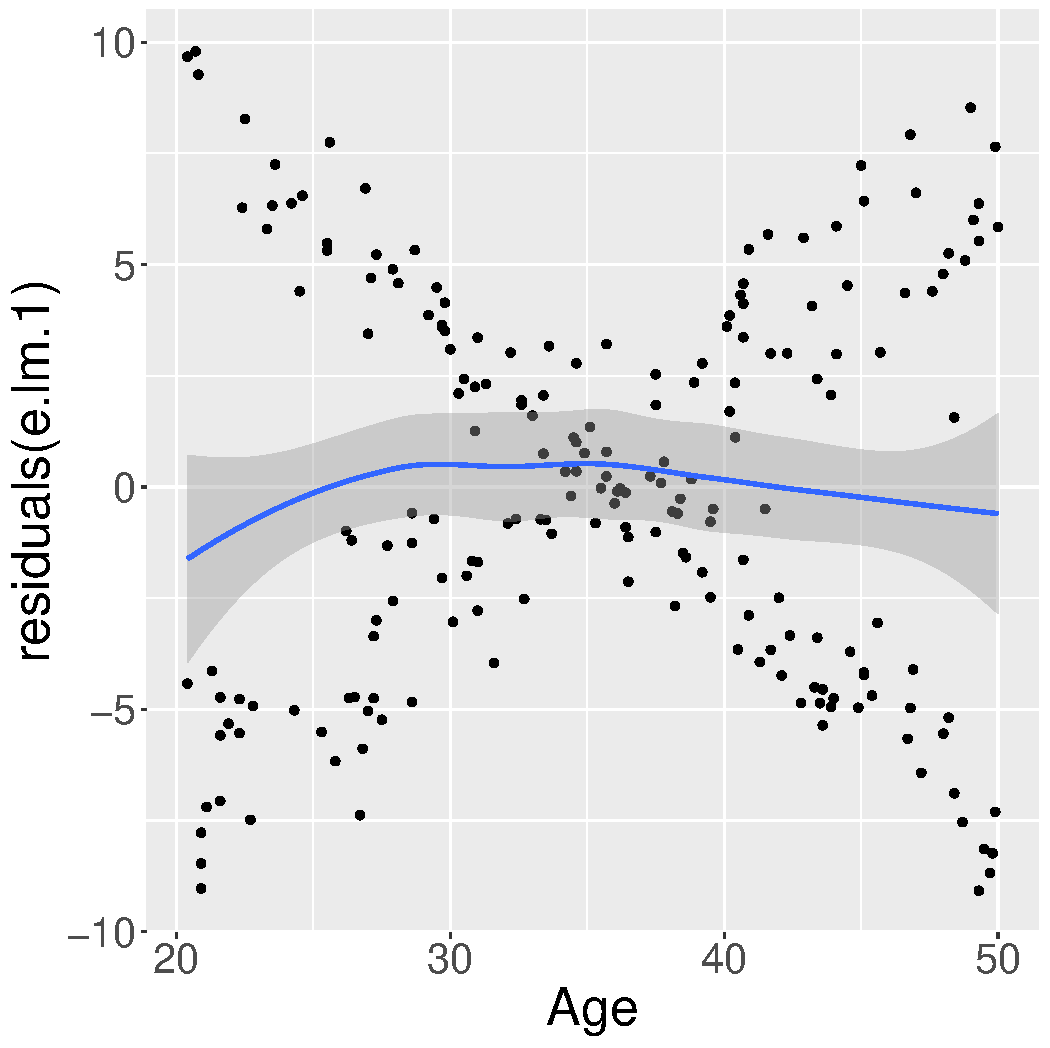
\includegraphics[width=1\textwidth]{./figures/A1-Age.pdf}
\end{center} 

\begin{itemize}
\item \textbf{checking for interactions} is hard because the number of possible
interactions grows quickly with the number of covariates. A typical
test would be to compare a model with interactions to a model
without interactions:
\end{itemize}
\lstset{language=r,label= ,caption= ,captionpos=b,numbers=none}
\begin{lstlisting}
e.lm.2 <- update(e.lm, Y ~ Gender*Age + Gene + BMI + I(BMI^2))
anova(e.lm.1, e.lm.2)
\end{lstlisting}

\begin{verbatim}
Analysis of Variance Table

Model 1: Y ~ Gender + Age + Gene + BMI + I(BMI^2)
Model 2: Y ~ Gender + Age + Gene + BMI + I(BMI^2) + Gender:Age
  Res.Df    RSS Df Sum of Sq      F    Pr(>F)    
1    193 4037.2                                  
2    192  318.7  1    3718.5 2240.4 < 2.2e-16 ***
---
Signif. codes:  0 '***' 0.001 '**' 0.01 '*' 0.05 '.' 0.1 ' ' 1
\end{verbatim}
Note that in that case a test on the cumulative residuals process
would not detect any issue:
\lstset{language=r,label= ,caption= ,captionpos=b,numbers=none}
\begin{lstlisting}
cumres(e.lm.1, variable = "predicted")
\end{lstlisting}

\begin{verbatim}

Kolmogorov-Smirnov-test: p-value=0.46
Cramer von Mises-test: p-value=0.642
Based on 1000 realizations. Cumulated residuals ordered by predicted-variable.
---
\end{verbatim}

\emph{Remedies}: this is a harder situation. When only few interactions are
considered, a possible strategy would be to include all of them and
perform backward selection. Otherwise adding all possible
interactions and use a group-lasso penalty, or use more flexible but
less interpretable models (e.g. random forest).

\bigskip

\begin{itemize}
\item A last possible issue arise when the \textbf{outcome variable is not
studied on the right scale}. Consider the model using a square root
transformation:
\end{itemize}
\lstset{language=r,label= ,caption= ,captionpos=b,numbers=none}
\begin{lstlisting}
e.sqrt.lm <- lm(sqrt(Y) ~ Gender*Age + Gene + BMI + I(BMI^2), data = d)
\end{lstlisting}

Diagnostic plots indicates lack of fit (first line, first plot) and
heteroschedasticity (second line first plot):
\lstset{language=r,label= ,caption= ,captionpos=b,numbers=none}
\begin{lstlisting}
autoplot(e.sqrt.lm)
## ggsave(autoplot(e.sqrt.lm) + theme(text = element_text(size=15)), filename = "./figures/A1-scale.pdf")
\end{lstlisting}

\begin{center}
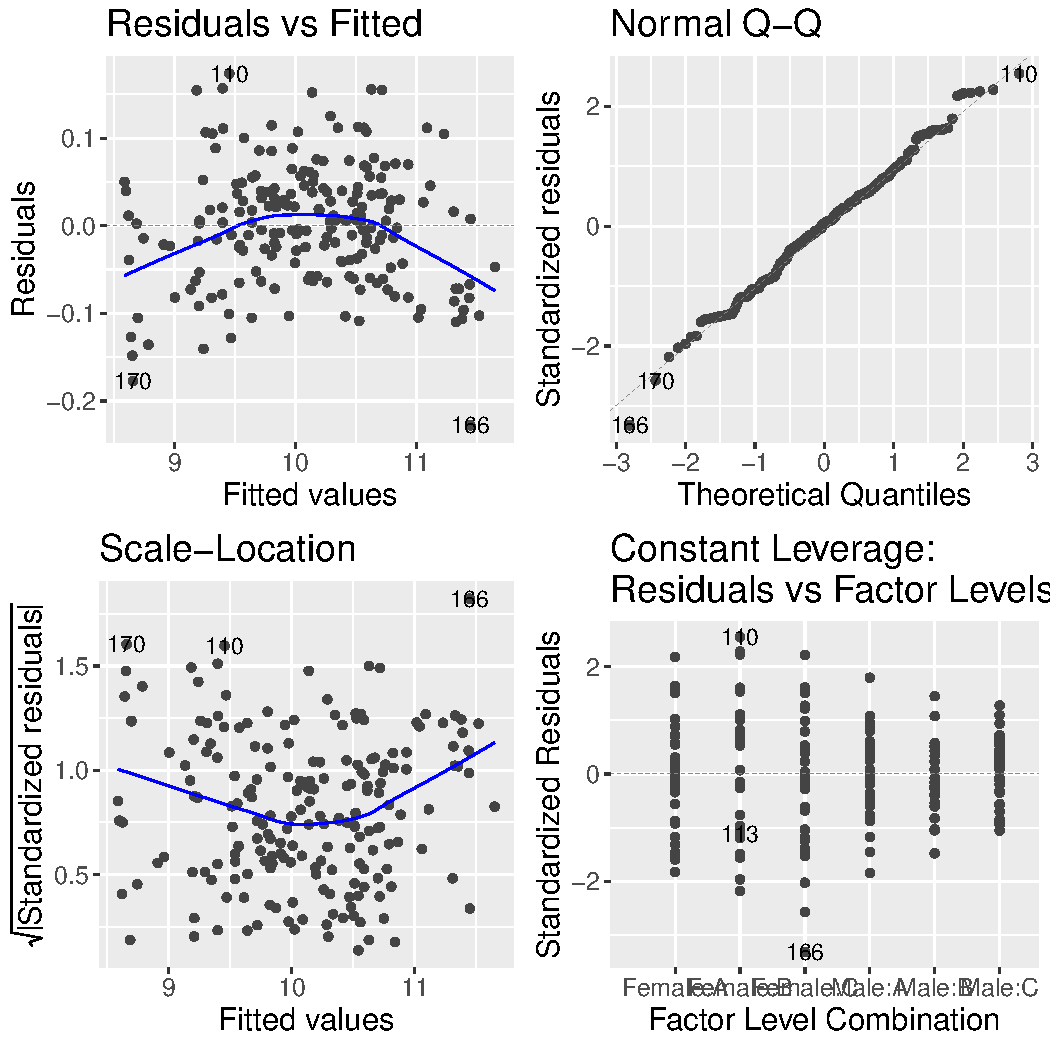
\includegraphics[width=1\textwidth]{./figures/A1-scale.pdf}
\end{center} 

We can use cumres and see that the link function seems inappropriate:
\lstset{language=r,label= ,caption= ,captionpos=b,numbers=none}
\begin{lstlisting}
cumres(e.sqrt.lm, variable = "predicted")
\end{lstlisting}

\begin{verbatim}

Kolmogorov-Smirnov-test: p-value=0.001
Cramer von Mises-test: p-value=0
Based on 1000 realizations. Cumulated residuals ordered by predicted-variable.
---
\end{verbatim}
In that case a box-cox transformation can be useful as it suggests to
square the outcome:
\lstset{language=r,label= ,caption= ,captionpos=b,numbers=none}
\begin{lstlisting}
M <- MASS::boxcox(e.sqrt.lm, lambda = seq(-1,4,by=0.1))
M$x[which.max(M$y)]
\end{lstlisting}

\begin{verbatim}
[1] 2.181818
\end{verbatim}

Note that it seems to sometimes also suggest weird transformations:
\lstset{language=r,label= ,caption= ,captionpos=b,numbers=none}
\begin{lstlisting}
M <- MASS::boxcox(lm(log(Y) ~ Gender*Age + Gene + BMI + I(BMI^2), data = d), lambda = seq(-10,10,by=0.1))
M$x[which.max(M$y)]
\end{lstlisting}

\begin{verbatim}
[1] 6
\end{verbatim}
(the results should be 0)

\subsection{\textbf{(A4)}: normal distribution}
\label{sec:orge4a2748}

\textbf{(A4)} can be tested using an histogram of the standardized residuals:
\lstset{language=r,label= ,caption= ,captionpos=b,numbers=none}
\begin{lstlisting}
hist(residuals(e.lm.2, type = "pearson"), freq = FALSE, breaks = 10)
curve(dnorm,-3,3,add =TRUE,col = "red")
\end{lstlisting}

\begin{center}
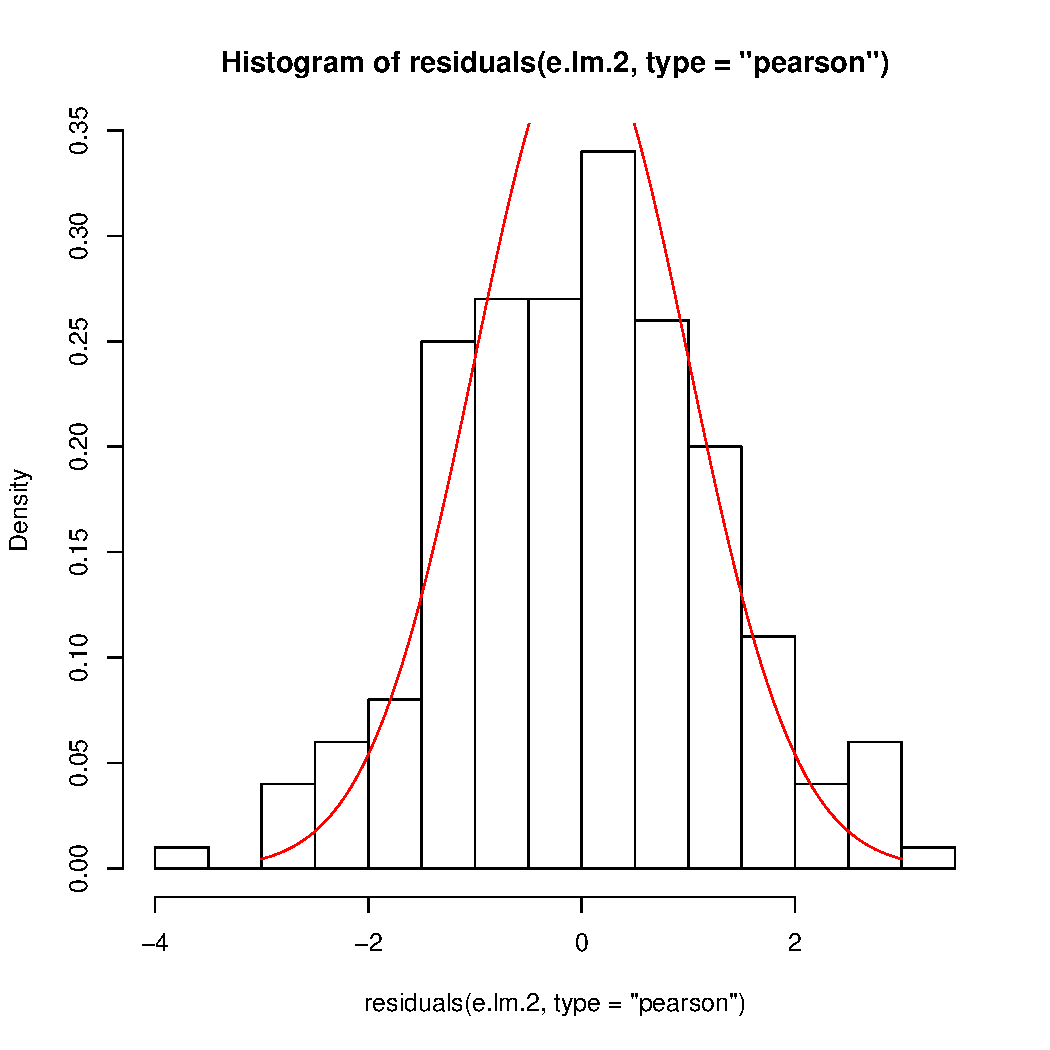
\includegraphics[width=.9\linewidth]{./figures/A4-hist-res.pdf}
\end{center}

where the histogram should be close to the shape of the standard
normal distribution (red curve). We could reject \textbf{(A4)} but accept
\textbf{(A4-bis)} in the case where the distribution has heavy tails but is
still unimodal and symmetric. While intuitive, this method is
sensitive to the discretization of the residuals values (argument
break) and a qq-plot is often preferred:
\lstset{language=r,label= ,caption= ,captionpos=b,numbers=none}
\begin{lstlisting}
qqtest::qqtest(residuals(e.lm.2, type = "pearson"))
\end{lstlisting}

\begin{verbatim}
00:00:00 left
\end{verbatim}

\begin{center}
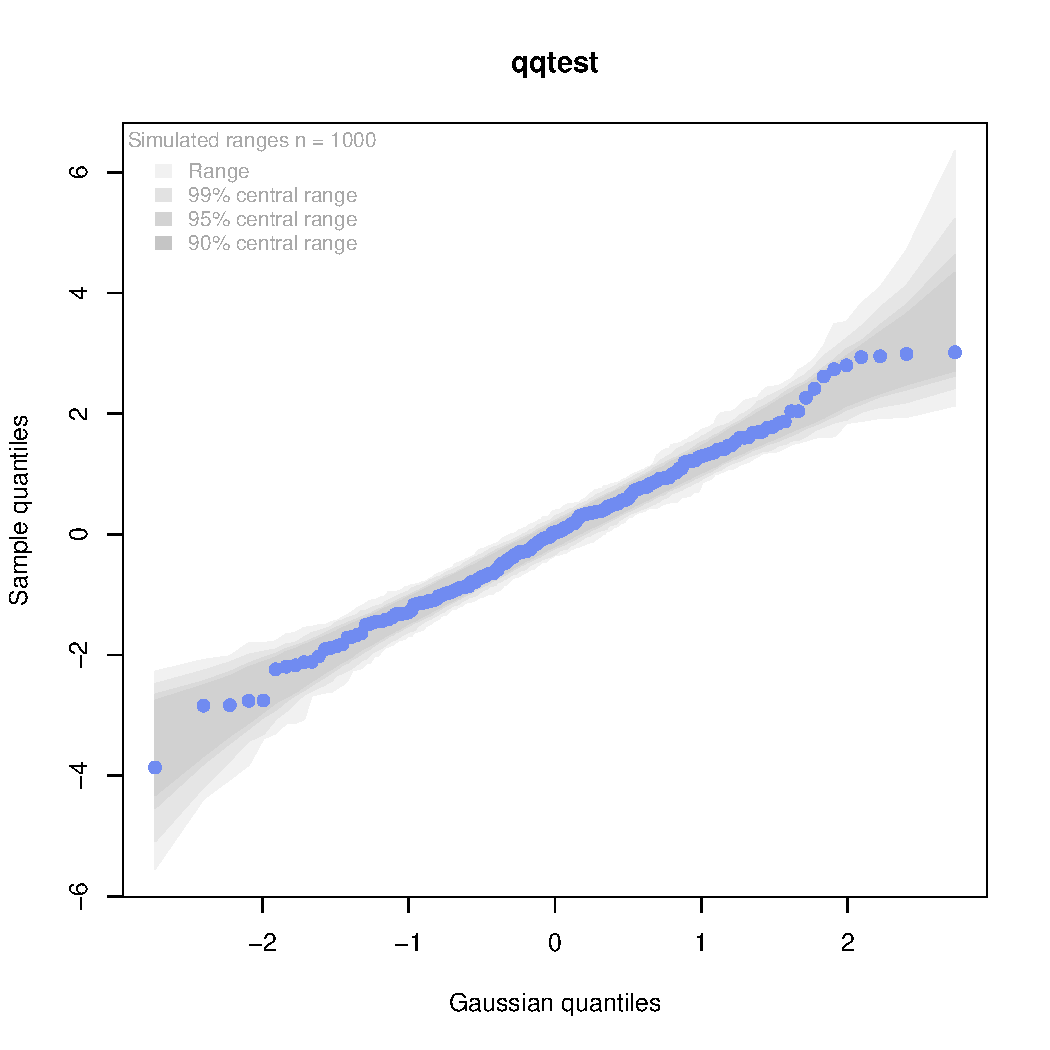
\includegraphics[width=.9\linewidth]{./figures/A4-qqplot-res.pdf}
\end{center}

Here the points should follow a straight line and be within the shaded
area. We could reject \textbf{(A4)} but accept \textbf{(A4-bis)} in the case where
deviation to the straight line mostly arise in the tails.  Statistical
test (like a shapiro test) are not recommended since they do not
enable us to know whether we reject \textbf{(A4)} or \textbf{(A4bis)}. 

\bigskip

\emph{Remedies}: when \textbf{(A4)} is rejected but not \textbf{(A4-bis)}, the main
concern is about the validity of the traditional asymptotic
results. This is not critical in a linear regression where our
variance estimator is consistent and the central limit theorem ensures
asymptotic normality: instead of having exact p-values/CI they are
only asymptotically valid. If the sample size is not too small they
will hold; otherwise permutation test are a good alternative. In more
complex models, robust standard errors or non-parametric bootstrap can
be used for large enough samples to obtain p-values/CI robust to
deviation to the normal distribution. \newline A more serious problem
arises when \textbf{(A4-bis)} is rejected. In that case one should consider
whether the expected outcome is really relevant. Alternative
approaches include transformation of the outcome or use of alternative
regression models (quantile regression, probability index models,
finite mixture models).

\bigskip

Note 1: the \texttt{type} argument indicates the type of residuals we want to
extract. Raw residuals are \(\hat{\varepsilon} = Y-\hat{Y}\), i.e. the
observed minus the fitted values. In models more complex than a
univariate linear regression, the raw residuals may not be iid. This
makes it difficult to assess the validity of the assumptions. In such
cases we display instead diagnostics for normalized residuals that, if
the assumptions of the model are correct, should follow a standard
normal distribution.

\bigskip

Note 2: an alternative to the \texttt{qqtest} function is the \texttt{qqPlot}
function from the car package.

\subsection{\textbf{(A2)}: Homeschedasticity}
\label{sec:org9ee8799}
Homoschedasticity can be inspected by displaying the residuals along
the fitted values:
\lstset{language=r,label= ,caption= ,captionpos=b,numbers=none}
\begin{lstlisting}
d$residuals <- residuals(e.lm.2, type = "pearson")
d$fitted <- fitted(e.lm.2)
gg <- ggplot(d, aes(x = fitted)) + ylab("residuals")
gg <- gg + geom_smooth(aes(y = residuals^2-1))
gg <- gg + geom_point(aes(y = residuals))
gg
## ggsave(gg + theme(text = element_text(size=25)), filename = "./figures/A2-smooth.pdf")
\end{lstlisting}

\begin{verbatim}
`geom_smooth()` using method = 'loess' and formula 'y ~ x'
\end{verbatim}

\begin{center}
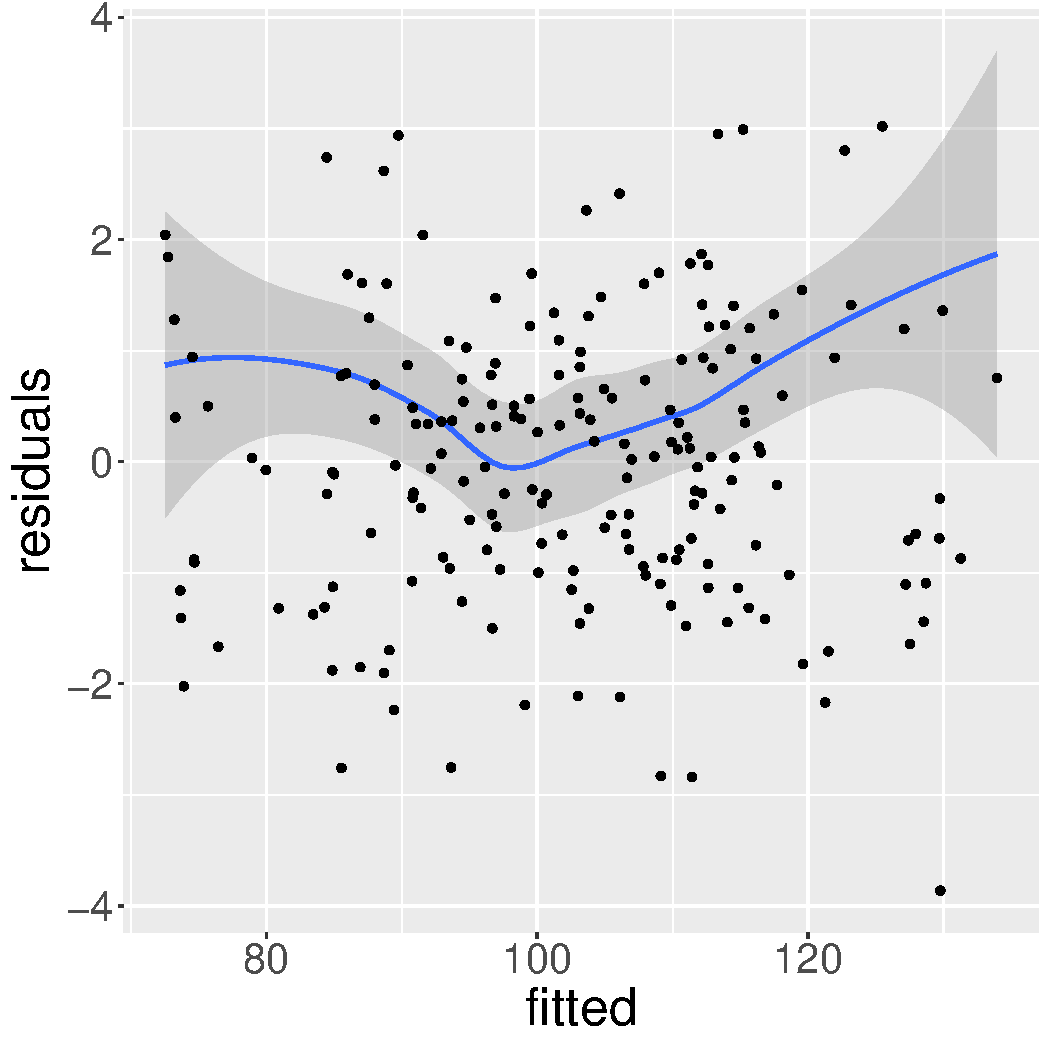
\includegraphics[width=.9\linewidth]{./figures/A2-smooth.pdf}
\end{center}

(see also the function \texttt{spreadLevelPlot} from the car package). It is
also possible to have a global statistical test (Breusch-Pagan test):
\lstset{language=r,label= ,caption= ,captionpos=b,numbers=none}
\begin{lstlisting}
ncvTest(e.lm.2)
\end{lstlisting}

\begin{verbatim}
Non-constant Variance Score Test 
Variance formula: ~ fitted.values 
Chisquare = 0.6009815, Df = 1, p = 0.4382
\end{verbatim}

Alternatively one can look along a specific regressor:
\lstset{language=r,label= ,caption= ,captionpos=b,numbers=none}
\begin{lstlisting}
gg <- ggplot(d, aes(x = Gender, y = residuals)) + ylab("residuals")
gg <- gg + geom_boxplot()
gg
## ggsave(gg + theme(text = element_text(size=25)), filename = "./figures/A2-boxplot.pdf")
\end{lstlisting}

\begin{center}
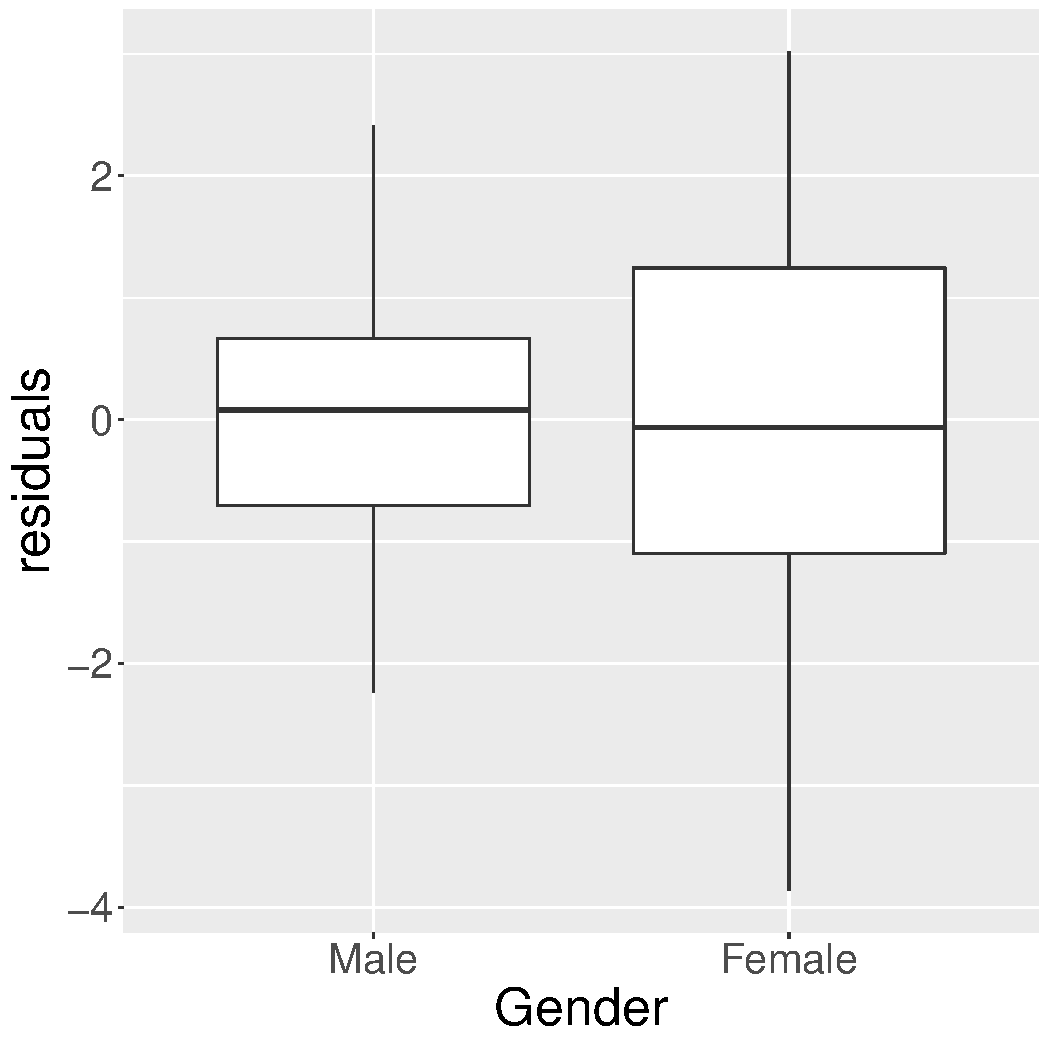
\includegraphics[width=.9\linewidth]{./figures/A2-boxplot.pdf}
\end{center}

or investigate look how the squared residuals relates to the
regressors:
\lstset{language=r,label= ,caption= ,captionpos=b,numbers=none}
\begin{lstlisting}
summary(lm(residuals(e.lm.2)^2 ~ Gender + Age + Gene + BMI, data = d))$coef
\end{lstlisting}

\begin{verbatim}
                Estimate Std. Error    t value     Pr(>|t|)
(Intercept)   6.45227607 3.65565988  1.7650100 7.913549e-02
GenderFemale  1.44221328 0.29848355  4.8318015 2.742530e-06
Age           0.01348642 0.01758548  0.7669068 4.440692e-01
GeneB         0.23754662 0.38188217  0.6220417 5.346448e-01
GeneC         0.03181216 0.34758915  0.0915223 9.271720e-01
BMI          -0.25529930 0.14902626 -1.7131161 8.828871e-02
\end{verbatim}

\emph{Remedies}: in presence of global heteroschadasticity (first graph),
transforming the outcome can be a solution. Otherwise one should
reflect about possible source of heteroschadasticity (e.g. correlated
observations, mixture of populations) and model them. When the
heteroschadasticity is related to a single variable, one can for
instance use the \texttt{gls} function to model this variance:
\lstset{language=r,label= ,caption= ,captionpos=b,numbers=none}
\begin{lstlisting}
e.gls <- gls(Y ~ Gender + Age + Gene + BMI + I(BMI^2) + Gender:Age, 
			 data = d,
			 weight = varIdent(form=~1|Gender))
summary(e.gls$modelStruct)
\end{lstlisting}

\begin{verbatim}
Variance function:
 Structure: Different standard deviations per stratum
 Formula: ~1 | Gender 
 Parameter estimates:
    Male   Female 
1.000000 1.650464
\end{verbatim}

\lstset{language=r,label= ,caption= ,captionpos=b,numbers=none}
\begin{lstlisting}
summary(
	lm(residuals(e.gls, type = "normalized")^2 ~ Gender + Age + Gene + BMI, data = d)
)$coef
\end{lstlisting}

\begin{verbatim}
                 Estimate Std. Error     t value  Pr(>|t|)
(Intercept)   2.845507264 2.08650094  1.36376994 0.1742203
GenderFemale  0.015137857 0.17036219  0.08885691 0.9292873
Age           0.005236824 0.01003707  0.52174821 0.6024408
GeneB         0.068737967 0.21796270  0.31536573 0.7528230
GeneC        -0.069620340 0.19838965 -0.35092728 0.7260237
BMI          -0.086243866 0.08505809 -1.01394080 0.3118739
\end{verbatim}


\subsection{\textbf{(A5)}: Influential observations}
\label{sec:org831fb7d}

The \texttt{influence} method can be used to output what is the impact of
each observation on each estimated parameter:
\lstset{language=r,label= ,caption= ,captionpos=b,numbers=none}
\begin{lstlisting}
if.lme <- influence(e.lm.2)
if.lme$coefficient[1:6,1:4]
\end{lstlisting}

\begin{verbatim}
  (Intercept) GenderFemale           Age         GeneB
1  0.03478943  0.018050611  6.597433e-04 -5.046560e-03
2 -0.05849442  0.001113552  4.583238e-05  9.488884e-04
3 -0.97841870 -0.018612231 -1.105912e-03  1.833443e-02
4  0.33314244  0.004040188  3.325704e-06 -2.090461e-05
5  0.34719463 -0.020540159 -4.416311e-04 -4.518752e-03
6 -0.33837887 -0.014621030 -3.528092e-04  1.299324e-04
\end{verbatim}

Here the value in the first line and third column indicates by how
much is changed the Age effect when removing the first observation.
\lstset{language=r,label= ,caption= ,captionpos=b,numbers=none}
\begin{lstlisting}
coef(update(e.lm.2,data=d[-1,]))-coef(e.lm.2)
\end{lstlisting}

\begin{verbatim}
  (Intercept)     GenderFemale              Age            GeneB            GeneC 
-0.0347894306    -0.0180506110    -0.0006597433     0.0050465601     0.0049566971 
          BMI         I(BMI^2) GenderFemale:Age 
 0.0063071805    -0.0001723731     0.0005968902
\end{verbatim}

Large values (positive or negative) indicate influential
observations. The following plot displaying in red the coefficient
value and in black the influence of each individual can be useful:
\lstset{language=r,label= ,caption= ,captionpos=b,numbers=none}
\begin{lstlisting}
dfW1.gg <- data.frame(id = "true", as.data.frame(t(coef(e.lm.2))))
dfW2.gg <- data.frame(id = as.character(1:NROW(d)), if.lme$coefficient)
dfL1.gg <- reshape2::melt(dfW1.gg, id.vars = "id")
dfL2.gg <- reshape2::melt(dfW2.gg, id.vars = "id")
gg.inf <-  ggplot() + facet_wrap(~variable, scales = "free")
gg.inf <- gg.inf + geom_boxplot(data = dfL2.gg, aes(y = value))
gg.inf <- gg.inf + geom_hline(data = dfL1.gg, aes(yintercept = value), color = "red")
gg.inf
## ggsave(gg.inf, filename = "./figures/A5-boxplot.pdf")
\end{lstlisting}

\begin{center}
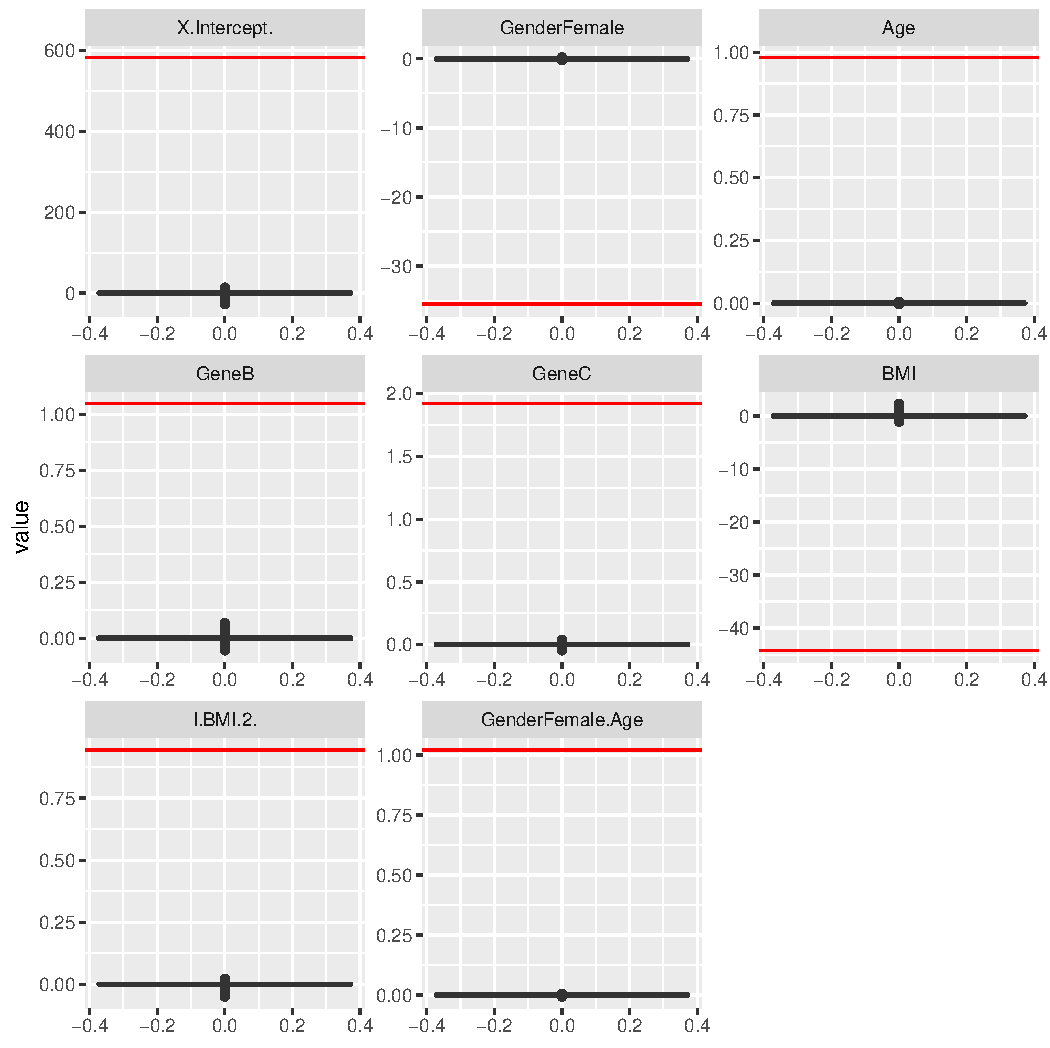
\includegraphics[width=.9\linewidth]{./figures/A5-boxplot.pdf}
\end{center}

When the aim is to perform prediction, global influence metrics such
as Cook's distance can be useful:
\lstset{language=r,label= ,caption= ,captionpos=b,numbers=none}
\begin{lstlisting}
autoplot(e.lm.2, which = 4)
## ggsave(autoplot(e.lm.2, which = 4), filename = "./figures/A5-cook.pdf")
\end{lstlisting}

\begin{center}
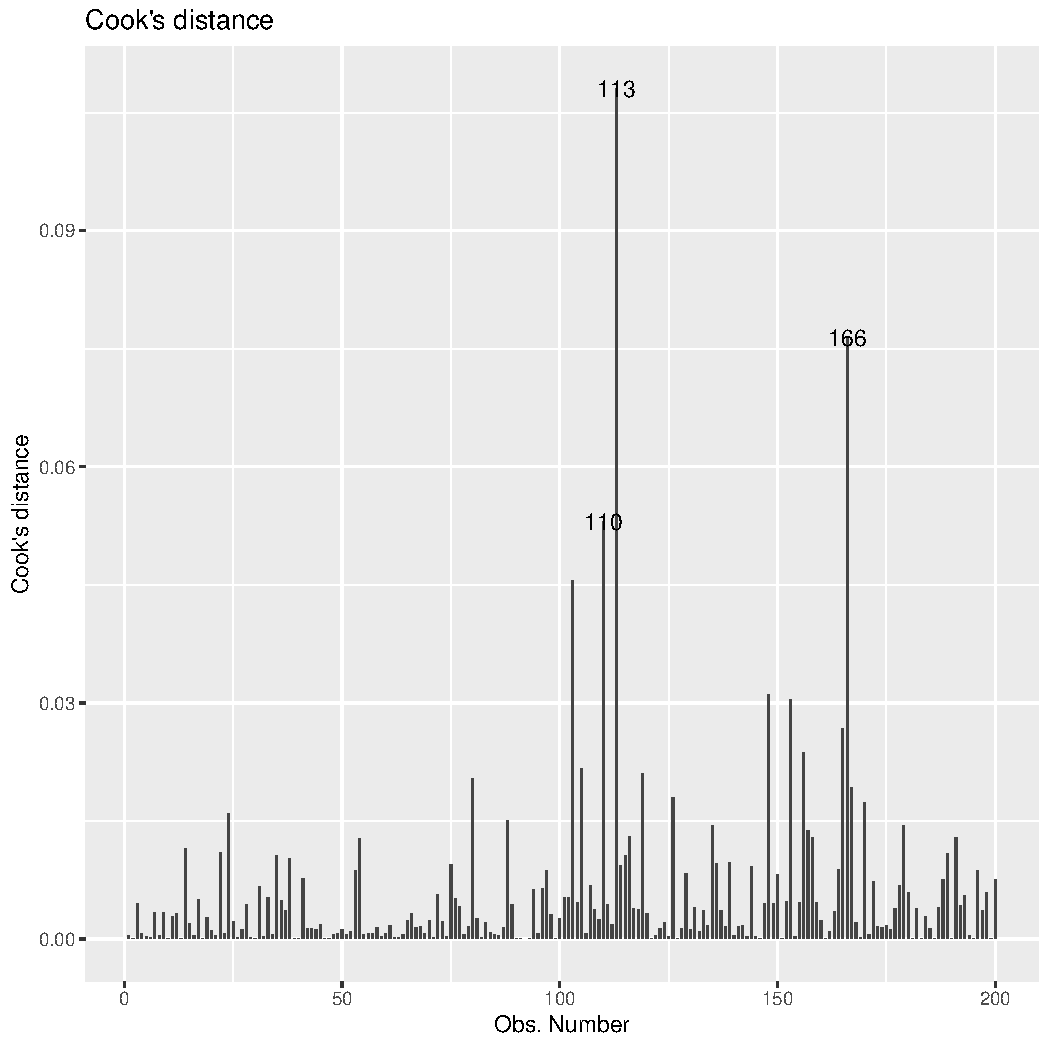
\includegraphics[width=.9\linewidth]{./figures/A5-cook.pdf}
\end{center}


\subsection{Others [no recommanded unless specific reasons]}
\label{sec:orga02ad59}
Some people recommand to check the correlation between the explanatory
variables, with the argument that when very correlated it is difficult
to disantangle effects and thus to interpret the regression
coefficients. The VIF (variance inflation factor) is typically
recommanded to check that with values higher than 5 considered as
high:

\lstset{language=r,label= ,caption= ,captionpos=b,numbers=none}
\begin{lstlisting}
car::vif(e.lm.2)
\end{lstlisting}

\begin{verbatim}
                  GVIF Df GVIF^(1/(2*Df))
Gender       18.757045  1        4.330940
Age           2.210228  1        1.486683
Gene          1.026260  2        1.006501
BMI        1031.164279  1       32.111747
I(BMI^2)   1031.061224  1       32.110142
Gender:Age   19.413821  1        4.406112
\end{verbatim}

I personnally don't recommand this as an automatic check since in many
  settings co-linearity can be better assessed from the meaning of the
  variables than from a statistical test. It is also quite unclear to
  me why 5 is a good cut-off and we see in this example that we get
  values close to five (or higher) even though there is no issue.

\clearpage

\section{Partial residuals}
\label{sec:org1453ff5}
\subsection{With respect to one variable}
\label{sec:org13a4605}

The partial residuals with respect to age are defined by removing the
effect of all the covariates but age on the outcome:
\begin{align*}
\hat{\varepsilon}^{Age}_i &= Y_i - \left(\alpha + \beta_{Gender} \Ind[Gender_i="Female"] + \beta_{GeneB} \Ind[Gene_i="B"] + \beta_{GeneC} \Ind[Gene_i="C"]  + \beta_{BMI} BMI_i\right)
\end{align*}
So for instance for the first individual:
\begin{align*}
\hat{\varepsilon}^{Age}_1 &= 115.7 - \left(21.3988 + 0.9778 * 0 + 1.3783 * 0 + 2.6682 * 0 + 1.0351 * 25.2\right) \\
                         &= 115.7 - 47.48 = 68.22
\end{align*}
At the dataset level, this type of partial residual is centered around
the expected value of the covariate times its effect (here
\(0.9814*36.078 \approx 35\)). These partial residuals can be
computed using the \texttt{partialResidual} function from the butils package:
\lstset{language=r,label= ,caption= ,captionpos=b,numbers=none}
\begin{lstlisting}
pRes.noI <- partialResiduals(e.lm, var = "Age", keep.intercept = FALSE)
head(pRes.noI)
\end{lstlisting}

\begin{verbatim}
       Y Gene  Age  BMI Id Gender     pFit ranef pResiduals
1: 115.7    A 48.0 25.2  1   Male 47.48357     0   68.21643
2: 108.7    B 42.4 24.3  2   Male 47.93024     0   60.76976
3: 108.6    A 41.7 25.4  3   Male 47.69059     0   60.90941
4: 104.4    C 36.4 24.9  4   Male 49.84120     0   54.55880
5:  93.3    A 27.9 22.9  5   Male 45.10282     0   48.19718
6:  97.3    C 29.2 24.5  6   Male 49.42716     0   47.87284
\end{verbatim}

or manually:
\lstset{language=r,label= ,caption= ,captionpos=b,numbers=none}
\begin{lstlisting}
keep.coef <- c("(Intercept)","GenderFemale","GeneB","GeneC","BMI")
d$Y[1] - model.matrix(e.lm)[1,keep.coef] %*% coef(e.lm)[keep.coef]
\end{lstlisting}

\begin{verbatim}
         [,1]
[1,] 68.21643
\end{verbatim}

A graphical display can be obtained using the \texttt{autoplot} function
(require the ggplot2 package):
\lstset{language=r,label= ,caption= ,captionpos=b,numbers=none}
\begin{lstlisting}
gg <- autoplot(pRes.noI)
## ggsave(gg + theme(text = element_text(size=25)), filename = "./figures/fig-butils-plotConf-noI.pdf")
\end{lstlisting}

\begin{center}
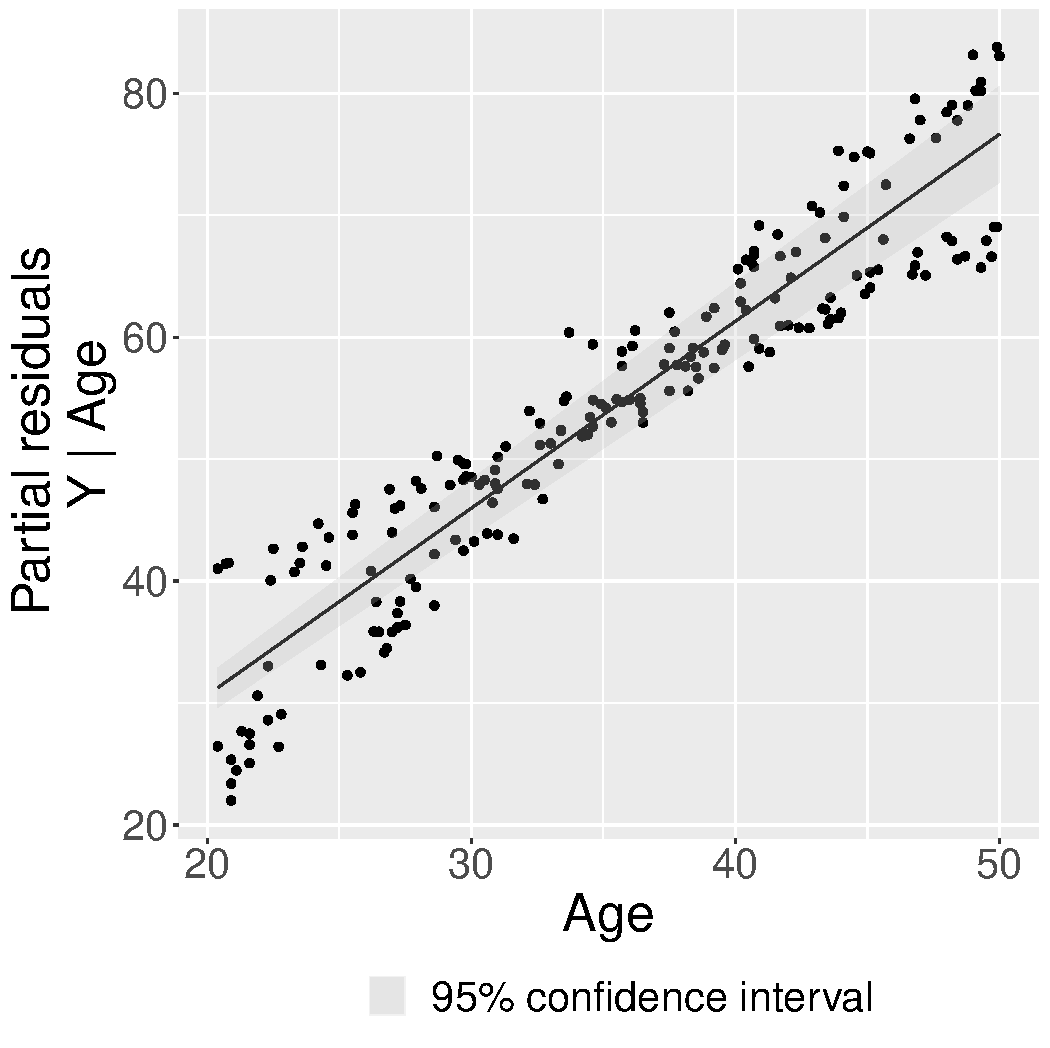
\includegraphics[width=0.7\textwidth]{./figures/fig-butils-plotConf-noI.pdf}
\end{center}

\begin{itemize}
\item An alternative definition do not remove the intercept effect:
\end{itemize}
\begin{align*}
\hat{\varepsilon}^{Age,\alpha}_i &= Y_i - \left(\beta_{Gender} \Ind[Gender_i="Female"] + \beta_{GeneB} \Ind[Gene_i="B"] + \beta_{GeneC} \Ind[Gene_i="C"] + \beta_{BMI} BMI_i \right)
\end{align*}
so now the residuals are centered around the intercept plus the
expected value of age times the age effect (here approximately 0). As
before the partial residuals can either be obtained via the
\texttt{partialResiduals} function:
\lstset{language=r,label= ,caption= ,captionpos=b,numbers=none}
\begin{lstlisting}
pRes.I <- partialResiduals(e.lm, var = "Age", keep.intercept = TRUE)
head(pRes.I)
\end{lstlisting}

\begin{verbatim}
       Y Gene  Age  BMI Id Gender     pFit ranef pResiduals
1: 115.7    A 48.0 25.2  1   Male 26.08478     0   89.61522
2: 108.7    B 42.4 24.3  2   Male 26.53145     0   82.16855
3: 108.6    A 41.7 25.4  3   Male 26.29181     0   82.30819
4: 104.4    C 36.4 24.9  4   Male 28.44242     0   75.95758
5:  93.3    A 27.9 22.9  5   Male 23.70403     0   69.59597
6:  97.3    C 29.2 24.5  6   Male 28.02837     0   69.27163
\end{verbatim}

or manually: 
\lstset{language=r,label= ,caption= ,captionpos=b,numbers=none}
\begin{lstlisting}
keep.coef <- c("GenderFemale","GeneB","GeneC","BMI")
d$Y[1] - model.matrix(e.lm)[1,keep.coef] %*% coef(e.lm)[keep.coef]
\end{lstlisting}

\begin{verbatim}
         [,1]
[1,] 89.61522
\end{verbatim}

This corresponds to what the \texttt{plotConf} function is displaying (R
package lava available on CRAN):
\lstset{language=r,label= ,caption= ,captionpos=b,numbers=none}
\begin{lstlisting}
lava::plotConf(e.lm, var1 = "Age")
\end{lstlisting}

\begin{center}
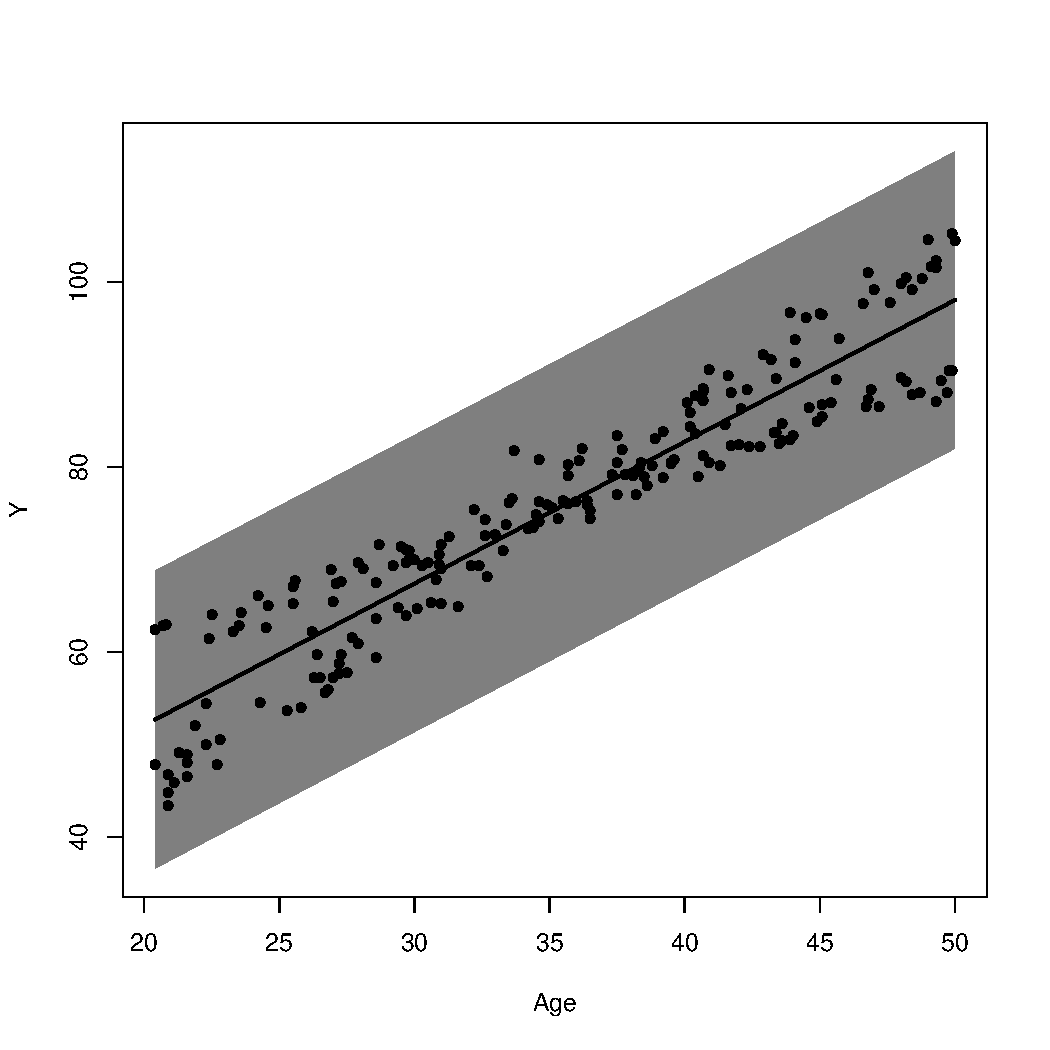
\includegraphics[width=.9\linewidth]{./figures/fig-lava-plotConf.pdf}
\end{center}

Note that it is also possible to display the partial residuals for a
categorical variable:
\lstset{language=r,label= ,caption= ,captionpos=b,numbers=none}
\begin{lstlisting}
gg <- autoplot(partialResiduals(e.lm, var = "Gene", keep.intercept = TRUE))
gg
## ggsave(gg + theme(text = element_text(size=25)), filename = "./figures/fig-butils-plotConf-categorical.pdf")
\end{lstlisting}

\begin{center}
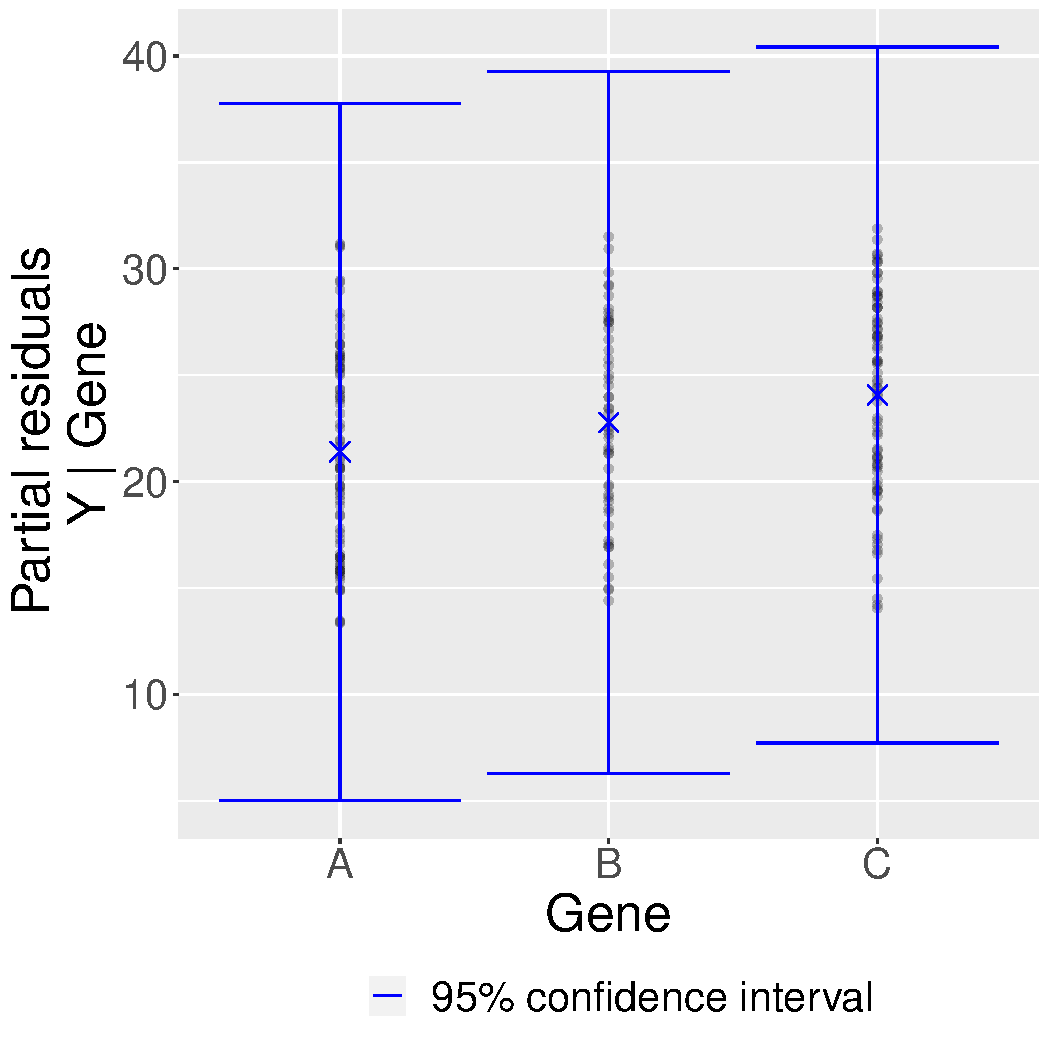
\includegraphics[width=1\textwidth]{./figures/fig-butils-plotConf-categorical.pdf}
\end{center}

\clearpage

\subsection{With respect to an interaction between two variables (one continuous, one categorical)}
\label{sec:org99df8f9}

Consider now a model where the age effect can be different for males
and females:
\lstset{language=r,label= ,caption= ,captionpos=b,numbers=none}
\begin{lstlisting}
e.lmI <- lm(Y~Gender*Age+Gene+BMI, data = d)
\end{lstlisting}

The partial residuals can be defined in a similar way as before. Here
the effect of Age and Gender (and their interaction) are not
substracted from the outcome:
\lstset{language=r,label= ,caption= ,captionpos=b,numbers=none}
\begin{lstlisting}
gg <- autoplot(partialResiduals(e.lmI, var = c("Age","Gender")))
## ggsave(gg + theme(text = element_text(size=25)), filename = "./figures/fig-butils-plotConf-interaction.pdf")
\end{lstlisting}

\begin{center}
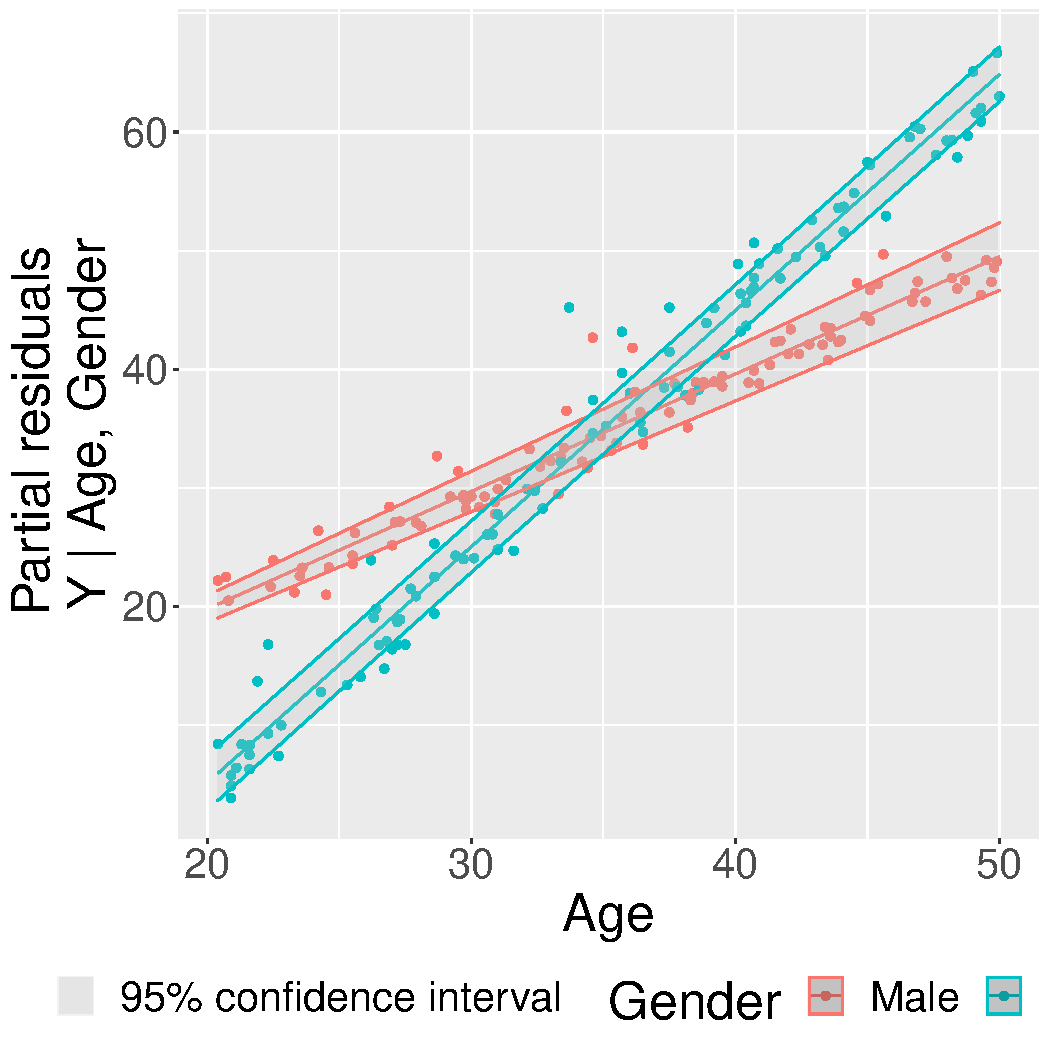
\includegraphics[width=0.7\textwidth]{./figures/fig-butils-plotConf-interaction.pdf}
\end{center}

\clearpage

\subsection{Customizing a partial residual plot}
\label{sec:orgd68211a}

The autoplot function returns the ggplot object:
\lstset{language=r,label= ,caption= ,captionpos=b,numbers=none}
\begin{lstlisting}
gg <- autoplot(partialResiduals(e.lm, var = "Gene", keep.intercept = TRUE))
class(gg)
\end{lstlisting}

\begin{verbatim}
[1] "gg"     "ggplot"
\end{verbatim}

So it can be easily customized, e.g. the text can be made bigger by
doing:
\lstset{language=r,label= ,caption= ,captionpos=b,numbers=none}
\begin{lstlisting}
gg + theme(text = element_text(size=25))
\end{lstlisting}
\end{document}